\documentclass{article}%
\usepackage[T1]{fontenc}%
\usepackage[utf8]{inputenc}%
\usepackage{lmodern}%
\usepackage{textcomp}%
\usepackage{lastpage}%
\usepackage[head=40pt,margin=0.5in,bottom=0.6in]{geometry}%
\usepackage{graphicx}%
%
\title{\textbf{Ministro alemán: Presencia de diplomáticos extranjeros impidió el arresto de Guaidó en el aeropuerto}}%
\author{AP}%
\date{07/03/2019}%
%
\begin{document}%
\normalsize%
\maketitle%
\textbf{URL: }%
http://www.eluniversal.com/politica/34979/ministro{-}aleman{-}presencia{-}de{-}embajadores{-}impidio{-}el{-}arresto{-}de{-}guaido{-}en{-}el{-}aeropuerto\newline%
%
\textbf{Periodico: }%
EU, %
ID: %
34979, %
Seccion: %
politica\newline%
%
\textbf{Palabras Claves: }%
NO\_TIENE\newline%
%
\textbf{Derecho: }%
2.1%
, Otros Derechos: %
\newline%
%
\textbf{\textit{El ministro Heiko Maas indicó que le pidió al embajador alémán, Daniel Kriener, que se sumara a otros enviados al aeropuerto porque existía información sobre intenciones de arrestar a Guaidó}}%
\newline%
\newline%
%
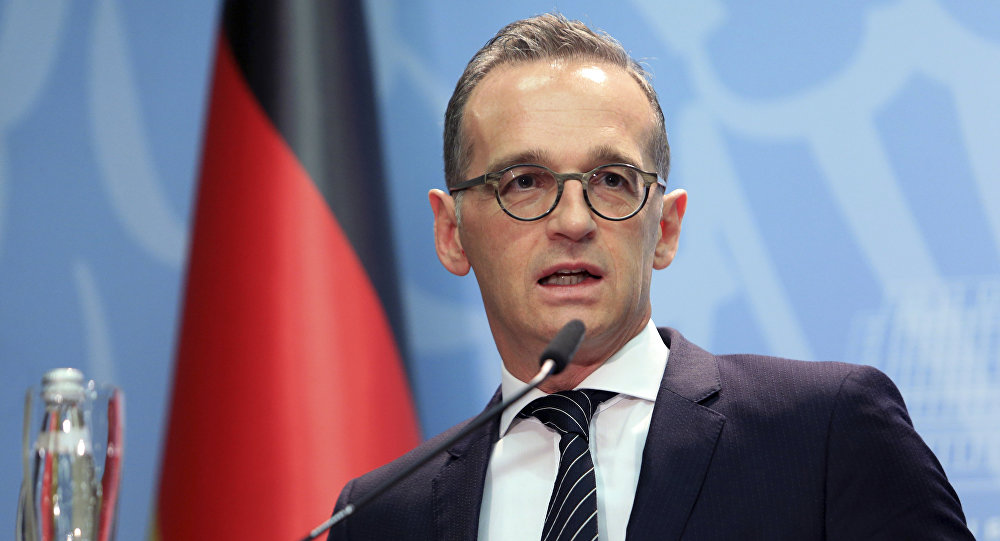
\includegraphics[width=300px]{EU_34979.jpg}%
\newline%
%
Berlín.{-} La presencia de diplomáticos extranjeros en el aeropuerto de Caracas a principios de esta semana ayudó a impedir el arresto del jefe legislativo, Juan Guaidó, dijo el ministro del Exterior alemán, Heiko Maas, este jueves.%
\newline%
%
Señaló que pidió al embajador alemán Daniel Kriener que se sumara a otros enviados en el aeropuerto el lunes. "Había información de que existían intenciones de arrestar (a Guaidó) allí, y creo que la presencia de varios embajadores ayudó a impedir este arresto".%
\newline%
%
El miércoles, el Gobierno de Nicolás Maduro anunció que le daba a Kriener 48 para abandonar el país, medida considerada una represalia por el apoyo de Alemania a Guaidó.%
\newline%
%
Maas dijo que "la decisión del gobierno venezolano, mejor dicho, el régimen de Maduro en Caracas, de expulsar al embajador Kriener como 'persona non grata' no es en absoluto algo comprensible o aceptable para nosotros".%
\newline%
%
Añadió que Alemania seguirá reconociendo a Guaidó como presidente interino legítimo de Venezuela y lo apoyará en la realización de elecciones.%
\newline%
%
\end{document}